% !TeX root = main.tex
\label{sec:setting}
\subsection{The net and the vacuum}
Let $H=L^2(\mathbb R;\mathbb C^r)$ and let $P_+$ be the Hardy projection.  With the
Fourier convention $\widehat f(k)=\int f(x)e^{-ikx}\,dx$, under which $P_+$ is the
projection onto $\{k<0\}$ --- the positive-energy subspace for the light-ray
coordinate used here --- its distributional kernel is
\begin{equation}\label{eq:hardy}
 P_+(x,y)=\tfrac12\delta(x-y)-\frac{i}{2\pi}\,\mathrm{p.v.}\frac1{x-y}.
\end{equation}
For a bounded interval $X$ write $E_X$ for multiplication by $\mathbf 1_X$ and
\begin{equation}\label{eq:QX}
 Q_X=E_XP_+E_X\big|_{L^2(X;\mathbb C^r)} .
\end{equation}
The net is $\cF_r(X)=\mathrm{CAR}\bigl(L^2(X;\mathbb C^r)\bigr)''$ in the vacuum
representation, i.e.\ $r$ complex chiral free fermions; its central charge is
$c_{\rm cft}=r$.  The vacuum restricted to $\cF_r(X)$ is the gauge-invariant
quasi-free state with symbol $Q_X$,
\begin{equation}\label{eq:qf}
 \omega\bigl(a^*(f)a(g)\bigr)=\langle g,Q_Xf\rangle .
\end{equation}
This is the net $\cA_r$ used by Longo and Xu \cite{LX}.  We use throughout:
\begin{enumerate}[label=(N\arabic*)]
\item the vacuum modular group of an interval algebra is the M\"obius subgroup
preserving that interval (Brunetti--Guido--Longo \cite{BGL});
\item an inclusion of interval algebras with one common endpoint is half-sided
modular, with the Borchers translations of Wiesbrock's theory \cite{Wiesbrock};
\item quasi-free CAR representations with symbols $S,T$ are quasi-equivalent iff
$S^{1/2}-T^{1/2}$ and $(1-S)^{1/2}-(1-T)^{1/2}$ are Hilbert--Schmidt
(Powers--St\o rmer \cite{PS70}, Araki \cite{ArakiCAR}).
\end{enumerate}

\subsection{Geometry}
Fix $a,b,c>0$ and put
\begin{equation}\label{eq:geometry}
 A=(-a,0),\quad B=(0,b),\quad C=(b,b+c),\quad D=BC=(0,L),\quad I=ABC=(-a,L),
\end{equation}
with $L=b+c$.  As in \cite{LX}, the endpoint-completed unions
$AB=(-a,b)$, $BC=(0,L)$, $ABC=(-a,L)$ are understood through the singular
inside-limit; under strong additivity, which holds for $\cF_r$, they agree with
the interval algebras.  We write
\begin{equation}\label{eq:eta-z}
 \eta=\frac{b(a+b+c)}{(a+b)(b+c)}\in(0,1),\qquad
 z=\frac1\eta-1=\frac{ac}{b(a+b+c)} .
\end{equation}
The letter $c$ denotes the length of the third interval; the central charge is
written $c_{\rm cft}$ whenever confusion is possible.

\begin{center}
\begin{tikzpicture}[x=1.05cm,y=0.7cm]
 \draw[->] (-4.6,0) -- (6.4,0) node[right] {$x$};
 \foreach \x/\l in {-3.6/{-a}, 0/{0}, 1.8/{b}, 4.6/{L=b+c}}
   \draw (\x,0.12) -- (\x,-0.12) node[below=1pt] {\footnotesize $\l$};
 \draw[very thick] (-3.6,0.55) -- (0,0.55) node[midway,above] {\footnotesize $A$};
 \draw[very thick] (0,0.55) -- (1.8,0.55) node[midway,above] {\footnotesize $B$};
 \draw[very thick] (1.8,0.55) -- (4.6,0.55) node[midway,above] {\footnotesize $C$};
 \draw[thick,dashed] (-3.6,-0.9) -- (2.9,-0.9)
   node[midway,below] {\footnotesize $J_s=\bigl(-a,\tfrac L{1+s}\bigr)$};
 \draw[->,thick] (4.55,0.25) .. controls (4.0,-0.35) and (3.4,-0.55) .. (2.95,-0.85);
\end{tikzpicture}
\end{center}
\noindent The recovery map compresses $I=ABC=(-a,L)$ onto $J_s\subset AB$, fixing
$A$ pointwise and pushing the right endpoint $L$ to $L/(1+s)$; for $s=\lambda=c/b$
one has $J_\lambda=AB$ exactly.

\subsection{The Longo--Xu conditional mutual information}
For two separated intervals $I_1=(a_1,b_1)$, $I_2=(a_2,b_2)$ with $b_1<a_2$, the
Longo--Xu free-fermion mutual information is
\begin{equation}\label{eq:LX-MI}
 F_r(I_1,I_2)=\frac r6\log\frac{(a_2-a_1)(b_2-b_1)}{(a_2-b_1)(b_2-a_1)} .
\end{equation}
Longo and Xu define a generalized mutual information $F_{\cN}(AB,BC)$ for
overlapping regions through Araki relative entropy, prove that it is the limit of
ordinary finite-dimensional conditional mutual informations (hence
$\ge0$), and control the singular limit in which the gaps close.

\begin{theorem}[Longo--Xu; Note~1]\label{thm:LX}
Let $\cB\subset\cA_r$ be either $\cA_r$ itself, a finite-index subnet, or one of
the finite-index extensions treated after \cite[Thm.~4.2]{LX}, and assume strong
additivity.  Then for the adjacent configuration \eqref{eq:geometry} the vacuum
conditional mutual information is finite and equals
\begin{equation}\label{eq:CMI}
 I_\omega(A{:}C\mid B)=F_{\cN}(AB,BC)
 =\frac r6\log\frac{(a+b)(b+c)}{b(a+b+c)}
 =\frac r6\log(1+z)=-\frac r6\log\eta .
\end{equation}
\end{theorem}

\begin{proof}
This is the main result of Note~1 \cite{Note1}, assembled from \cite[Thm.~4.1(5),(6)
and Thm.~4.2]{LX}: the gap-regularized combination
$F_r(A_\eps,D)-F_r(A_\eps,B)$ is computed from \eqref{eq:LX-MI},
\begin{equation}\label{eq:delta-eps}
 \delta_\eps=\frac r6\log\frac{(L+\eps)(a+b)}{(b+\eps)(a+L)} ,
\end{equation}
and the endpoint divergence and the global-index constant cancel in the
conditional combination, so that $\eps\downarrow0$ gives \eqref{eq:CMI}.
Positivity is $(a+b)(b+c)-b(a+b+c)=ac>0$.
\end{proof}

\begin{remark}\label{rem:LX-scope}
The rigorous scope of \cref{thm:LX} is the free-fermion class just described.
Longo and Xu conjecture in their Remark~4.3 that the same formula holds for every
rational conformal net with $r$ replaced by the central charge; that broader claim
is not used here.  A full two-dimensional CFT needs a separate left--right
analysis, which is the subject of \cref{sec:2d}.
\end{remark}

\subsection{Conditional mutual information as a Markov defect}
In finite dimensions, $I_\omega(A{:}C\mid B)$ is exactly the loss of
distinguishability under the Petz map of the inclusion
$\cN=\cB(\mathcal H_{AB})\subset\cM=\cB(\mathcal H_{ABC})$, and it vanishes iff
$\omega$ is a quantum Markov chain, in which case the Petz map recovers
$\omega_{ABC}$ from $\omega_{AB}$ exactly (Petz \cite{Petz88}; see Note~2 \cite{Note2}, where
the hypothesis $D(\omega\Vert\widetilde\omega)<\infty$ needed in the
type III statement is made explicit).  The bound that survives in general is
\eqref{eq:fhsw}: for the rotated Petz maps $\alpha_t$ of \cite{FHSW} --- normal
unital $2$-positive maps, not necessarily channels in the naive sense --- the
recovery error is bounded by the conditional mutual information.  Combining
\eqref{eq:fhsw} with \eqref{eq:CMI} gives
\begin{equation}\label{eq:cmi-bound}
 -\log \Fid(\omega,\widetilde\omega)\ \le\ \tfrac r{12}\log(1+z),
\end{equation}
a bound linear in $z$ for small $z$.  Everything that follows is devoted to the
exact behaviour, which is quadratic.

